\chapter{Climate Knowledge in Large Language Models}

% **************************** Define Graphics Path **************************
\ifpdf
    \graphicspath{{Chapter4/Figs/}{Chapter4/Figs/PDF/}{Chapter4/Figs/}}
\else
    \graphicspath{{Chapter4/Figs/Vector/}{Chapter4/Figs/}}
\fi

\noindent\textit{Parts of this chapter are based on the work \emph{``Climate Knowledge in Large Language Models''}, by Kuznetsov, I., \textbf{Grassi, J.}, Pantiukhin, D., Shapkin, B., Jung, T., and Koldunov, N. The manuscript has been published in Artificial Intelligence for the Earth Systems, a journal of the American Meteorological Society.}

\vspace{0.5em}
\begin{center}
    \rule{0.5\textwidth}{0.4pt}
\end{center}
\vspace{0.5em}

The previous chapters examined how Artificial Intelligence can operate directly on numerical climate data: first by supporting their production through AI-based forecasting models, and then by extracting meaningful information from them through diagnostic Machine Learning methods. This and the following chapters moves to a different stage of the Climate Services value chain, where climate information must be organized, interpreted, and made accessible to users.

Large Language Models offer new possibilities at this stage. Their ability to interact through natural language may facilitate access to climate information for users with different levels of technical expertise. However, the fluency of their answers does not guarantee that the information they provide is accurate, traceable, or scientifically reliable. LLMs may generate responses using knowledge encoded in their parameters, retrieve information from external sources, or combine both mechanisms. Understanding the contribution and limitations of each component is therefore essential before these systems can be reliably integrated into Climate Services.

In this chapter, the focus is placed on the \emph{parametric knowledge} of LLMs: the information encoded in their parameters during training and available without access to external documents, datasets, or computational tools. This use of the term knowledge should be distinguished from the broader meaning adopted in the DIKW framework. While the latter refers to information interpreted and contextualized for a specific purpose, parametric knowledge describes what a language model can reproduce from its internal representation alone.

The central question addressed here is therefore: how accurately do LLMs represent quantitative climate information, and how does their reliability vary across locations and environmental conditions? To investigate this question, the chapter evaluates the ability of different LLMs to estimate historical temperature climatologies and observed warming across the globe. Their answers are compared with reference reanalysis data to assess geographical patterns, systematic biases, and the influence of the contextual information included in the prompts.

By establishing what LLMs can and cannot reliably provide in a closed-book setting, this chapter defines a baseline for their use in Climate Services. It also motivates the augmentation strategies examined in the following chapter, where language models are connected to external scientific literature, climate datasets, and analytical tools.

\section{Large Language Models as Interfaces to Climate Knowledge}

Climate Services do not consist solely of producing and distributing climate data. Their broader purpose is to mediate between scientific evidence and the users who need that evidence to understand risks, evaluate possible responses, and support decisions. This mediation requires the selection, interpretation, contextualization, and communication of information according to specific questions and user needs. Consequently, increasing the availability or resolution of climate data does not necessarily make climate information more accessible or usable \citep{findlater_climate_2021,doblas-reyes_linking_2021}.

Traditionally, this mediation has been provided through scientific reports, data portals, decision-support tools, and direct interaction with climate experts. Although these mechanisms remain essential, they often require users to identify appropriate sources, understand technical terminology, and navigate heterogeneous formats. Large Language Models introduce a different mode of interaction. By allowing users to formulate questions in natural language, they can potentially lower some of these technical barriers and provide a common interface to scientific documents, climate datasets, and model outputs.

LLMs act as an intermediate layer between available information and the user: they select, combine, reformulate, and present content in response to a question. This gives them the potential to support the transformation of climate information into more accessible and contextualized knowledge. At the same time, it introduces uncertainty about the origin and reliability of the generated answers. Understanding how these systems construct their responses is therefore a prerequisite for evaluating their possible contribution to Climate Services.


\subsection{From Climate Information to Climate Knowledge}

Within the DIKW framework adopted in this dissertation, information becomes knowledge when it is interpreted and connected to a specific context, question, or objective. Climate information may describe, for example, the historical temperature of a region, the projected change in precipitation, or the expected frequency of an extreme event. On its own, however, this information does not necessarily explain why the change is relevant, which activities may be affected, or how it should be interpreted by a particular user.

The transition from information to knowledge therefore involves more than the extraction of indicators from data. It requires the combination of different sources, the identification of relevant relationships, and the communication of results in a form that can be understood and interrogated. This process is particularly challenging in climate applications because the available evidence is distributed across scientific literature, observational records, reanalysis products, climate model simulations, and sector-specific studies. These sources differ in their spatial and temporal scales, assumptions, uncertainties, and intended audiences.

LLMs may support this transition in several ways. They can summarize scientific material, explain technical concepts, compare information from different sources, and adapt the form of an answer to the question posed by the user. Unlike static reports or conventional data portals, a conversational interface also enables an iterative interaction in which users can refine their questions, request clarification, or explore different aspects of the same problem. Recent climate-oriented assistants have therefore investigated the use of LLMs as interfaces to scientific literature and other climate information sources \citep{vaghefi_chatclimate_2023,koldunov_local_2024}.

Nevertheless, an answer expressed in accessible and coherent language cannot automatically be considered knowledge. LLMs generate text by modelling statistical relationships between linguistic elements, rather than by independently verifying the scientific validity of each statement. Their answers may omit relevant qualifications, combine information referring to different periods or locations, or express uncertain content with unjustified confidence. They may also provide little indication of the evidence on which a statement is based.

The contribution of LLMs to knowledge creation therefore depends not only on their ability to generate relevant text, but also on the reliability, provenance, and uncertainty of the information included in their answers. This makes it necessary to distinguish between information already encoded within the language model and information obtained from external and verifiable sources.


\subsection{Parametric Knowledge and External Knowledge Sources}

The information that an LLM acquires during training is commonly referred to as its \emph{parametric knowledge}. Rather than being stored as an explicit collection of documents or database entries, this information is represented implicitly through the parameters of the model. As a result, an LLM may reproduce factual information, geographical associations, or general climatic relationships without consulting an external source.

Parametric knowledge should not, however, be interpreted as a structured or authoritative database. The model generally cannot identify the specific source from which a piece of information originated, determine whether it remains current, or guarantee that different elements of an answer refer to consistent datasets and reference periods. Its representation of a topic also reflects the frequency, geographical coverage, and quality of the material included in its training data. Widely documented locations and general global patterns may therefore be represented more accurately than less documented regions or geographically specific climate conditions.

For climate applications, this distinction is particularly important. An LLM may have learned general relationships such as the decrease of temperature with latitude or elevation, the seasonal contrast between hemispheres, or the approximate magnitude of global warming. These associations may allow it to produce plausible estimates for many locations. Plausibility, however, does not ensure the precision required for quantitative assessments, especially when local climate is influenced by topography, coastal effects, land cover, or regional circulation patterns.

Alternatively, an LLM can be connected to external knowledge sources. Retrieval-augmented systems provide the model with relevant passages from scientific documents, while tool-based systems may allow it to query climate databases, process numerical data, or interact with model outputs \citep{lewis_retrieval-augmented_2020}. These approaches can provide access to more precise and traceable information, but they do not completely replace the model's parametric knowledge. The LLM must still formulate queries, interpret retrieved material, combine different results, and communicate them to the user. Moreover, retrieval or tool use may not be available in every deployment or may not be activated for every question.

Evaluating parametric knowledge separately therefore provides an important baseline. It makes it possible to determine which aspects of climate information are already represented within an LLM, where systematic errors arise, and when external sources become necessary. It also helps distinguish improvements produced by retrieval or analytical tools from the capabilities of the underlying language model.

The remainder of this chapter isolates this closed-book component by asking LLMs quantitative and geographically specific questions without providing external climate data. Their answers are compared with authoritative reference information to evaluate whether the models reproduce broad climatological patterns, how their accuracy varies across space and environmental conditions, and whether they capture observed changes in climate. This evaluation establishes the baseline against which the augmented systems considered in the following chapter can be assessed.

\section{Evaluating Parametric Climate Knowledge}

The evaluation was designed as a closed-book benchmark of quantitative climate knowledge. Rather than asking the models to discuss general climate concepts, we posed questions for which an objectively verifiable numerical answer could be obtained from an authoritative climate dataset. This makes it possible to evaluate not only whether the answers are plausible, but also how closely they reproduce the magnitude and spatial structure of the reference climate information.

The benchmark focuses on near-surface air temperature. Temperature was selected because it is a widely understood climate variable, is available globally from reanalysis products, and exhibits well-defined spatial and seasonal patterns. At the same time, its local value depends on several geographical factors, including latitude, elevation, continentality, and proximity to the coast. It therefore provides a simple but informative test of whether LLMs encode both broad climatic regularities and geographically specific information.


\subsection{Evaluation Questions}

The evaluation was organized around four related questions. First, we asked whether LLMs can reproduce the geographical distribution of a present-day temperature climatology. This provides a test of whether their parameters encode broad climatic patterns, such as the contrast between tropical and high-latitude regions, as well as more localized variations.

Second, we investigated whether the accuracy of this knowledge depends on the geographical context provided to the model. Coordinates provide an unambiguous representation of location, but they may not be the format through which geographical information is most commonly represented in the textual material used to train an LLM. Country, region, and city names may instead act as linguistic anchors connecting the question to information encountered during training. The benchmark therefore compares prompts containing coordinates and geographical descriptors with prompts containing coordinates alone.

Third, we examined whether the ability to represent temperature climatology extends across the annual cycle. The main experiment focuses on July, while a second experiment evaluates all twelve calendar months for a subset of locations and models. This makes it possible to determine whether the conclusions obtained for a single month generalize to different seasons and to both hemispheres.

Finally, we assessed whether LLMs can represent not only the mean state of the climate but also its temporal evolution. For this purpose, the models were asked to estimate the change in mean July temperature between two historical periods. This last experiment distinguishes the recall of relatively static climatological information from the ability to represent geographically differentiated patterns of observed climate change.


\subsection{Reference Climate Information}

Reference values were obtained from the ERA5 reanalysis, which provides a physically consistent reconstruction of the atmosphere by combining observations with a numerical weather prediction model \citep{hersbach_era5_2020}. ERA5 was used as the reference because of its global coverage, temporal consistency, and widespread use in climate applications. The comparison should nevertheless be interpreted as agreement with the reanalysis rather than with direct observations at each individual location.

A regular grid with a resolution of \(1^{\circ}\) in latitude and longitude was generated between \(60^{\circ}\,\mathrm{S}\) and \(85^{\circ}\,\mathrm{N}\), covering the full range of longitudes. Antarctica and the northernmost Arctic regions were therefore excluded. After removing ocean cells, the evaluation domain contained 15,395 land grid points.

For each point, the primary reference variable was the mean July 2-m air temperature over the 1991--2020 climatological period. This period corresponds to a standard 30-year climate normal and provides the target for the main closed-book experiment. The resulting field contains a broad range of climatic conditions and allows the models to be evaluated consistently across different continents, latitudes, and elevations.

Each grid point was also associated with the nearest available country, administrative region, and city using the Nominatim reverse-geocoding service \citep{nominatim_nominatim_2026}. These descriptors were not used to determine the reference temperature. Their purpose was to test whether expressing the same location through familiar geographical names helps the models access information encoded in their parameters.

To evaluate the seasonal cycle, the reference dataset was extended to include the 1991--2020 mean 2-m air temperature for all twelve calendar months. Because of the computational cost of repeatedly querying the models, this experiment was conducted on a subset of 1,540 land points, obtained by retaining every tenth point from the original grid.

The magnitude of the model errors across the annual cycle was also compared with the natural interannual variability represented by ERA5. For each grid point and calendar month, yearly temperature anomalies were calculated relative to the corresponding 1991--2020 monthly mean. The root-mean-square of these anomalies provides an observational reference for the typical year-to-year variation in monthly temperature. It is used only as a scale for interpreting the LLM errors and not as an evaluation metric for the models themselves.

Finally, the climate-change experiment considered the difference in mean July temperature between the periods 1950--1974 and 2000--2024:

\begin{equation}
    \Delta T_i =
    \overline{T}_{i,\,2000\text{--}2024}
    -
    \overline{T}_{i,\,1950\text{--}1974},
\end{equation}

where \(i\) identifies a land grid point. The same difference was calculated from ERA5 and used as the reference against which the estimates produced by the LLMs were evaluated.


\subsection{Language Models and Prompting Strategies}

The benchmark included both proprietary and open-weight language models, covering different model families, parameter counts, and levels of domain specialization. The evaluated models included the GPT-5 family, GPT-OSS 120B and 20B, Mistral-small-3.1 24B, Gemma 27B and 12B, Gemini-2.5-flash-lite, Llama3.1 8B, Mistral-nemo 12B, Llama2 70B, and the domain-adapted eci-io-climategpt 70B. Considering the different sampling configurations, the main experiment comprised 17 model configurations.

Open-weight models were run locally through Ollama. To support reproducibility, the specific model images, parameter counts, and quantization settings are reported in Table~\ref{tab:model_configurations}. Proprietary models were accessed through their respective providers. Since their internal weights and quantization schemes are not publicly available, their configurations are identified through the model names and versions exposed by the providers.

All models were evaluated in a closed-book setting. They were not given access to external documents, climate databases, web search, code execution, or computational tools. No few-shot examples or chain-of-thought instructions were provided. The intention was to isolate the information available from the parameters of the model rather than evaluate its ability to retrieve or calculate the requested values.

For the main experiment, each model received a standardized prompt requesting the mean July 2-m air temperature for the period 1991--2020 at a specified location. The prompt included latitude, longitude, country, administrative region, and nearest city when these descriptors were available. Models were instructed to return only a single numerical value in degrees Celsius. Restricting the output format reduced ambiguity and allowed the responses to be processed automatically.

The core structure of the prompt was:

\begin{quote}
\small
You are a climate data expert. Given the location coordinates and address information below, provide the mean July temperature for the period 1991--2020.

Location information:
longitude, latitude, country, state or region, and city.

Provide only the mean July temperature at 2 m above the surface in degrees Celsius. Return a single numerical value.
\end{quote}

A second version of the experiment removed the country, region, and city fields while leaving the coordinates unchanged. Comparing the two configurations isolates the contribution of textual geographical context and provides an indication of whether model responses are driven primarily by numerical coordinates or by associations with place names.

Each model was queried ten times for every location. If an individual request did not return a valid numerical response, that request was repeated up to three additional times. Non-numerical answers and values outside the physically plausible interval from \(-90\,^{\circ}\mathrm{C}\) to \(60\,^{\circ}\mathrm{C}\) were treated as invalid. The final prediction for a location was calculated as the mean of the ten valid responses.

Where supported by the model interface, the main experiment was performed using sampling temperatures of 0 and 0.3. The first setting produces more deterministic outputs, whereas the second permits limited variation between repeated queries. Additional experiments using the default sampling configuration of each provider were conducted on the reduced 1,540-point grid. These comparisons test whether the estimated climate knowledge is stable with respect to the randomness introduced during text generation.

For the seasonal experiment, the four best-performing model families from the July evaluation were asked to return the twelve monthly climatological temperatures in a single response. Answers were retained only when they contained twelve numerical and physically plausible values. The procedure was again repeated ten times at each location, and the mean of the valid responses was used in the evaluation.

The climate-change prompt followed the same structure as the climatological prompt but requested the difference between the 2000--2024 and 1950--1974 mean July temperatures. The models were explicitly instructed to return the later period minus the earlier period as a single value in degrees Celsius. This task remained closed-book: the models were not provided with the two underlying temperature fields or with any external time series from which the difference could be calculated.


\subsection{Evaluation Metrics}

Model predictions were compared point by point with the corresponding ERA5 values. Let \(\hat{T}_i\) denote the mean value returned by an LLM at location \(i\), and let \(T_i\) denote the ERA5 reference. The primary measure of accuracy was the root-mean-square error:

\begin{equation}
    \mathrm{RMSE} =
    \sqrt{
        \frac{1}{N}
        \sum_{i=1}^{N}
        \left(\hat{T}_i-T_i\right)^2
    }.
\end{equation}

RMSE was selected as the main metric because it measures the magnitude of point-wise errors and gives greater weight to locations with large deviations. Metrics were computed across the land grid without area weighting, as the objective was to evaluate the accuracy of an individual answer at each queried location rather than obtain a globally area-weighted climatic average.

The mean bias was calculated as:

\begin{equation}
    \mathrm{Bias} =
    \frac{1}{N}
    \sum_{i=1}^{N}
    \left(\hat{T}_i-T_i\right).
\end{equation}

Positive values indicate that the LLM produces temperatures that are warmer than ERA5 on average, while negative values indicate a cold tendency. Bias was treated as a complementary metric because errors with opposite signs can compensate when averaged over the full domain. A small global bias therefore does not necessarily imply accurate local or regional estimates.

The spatial distribution of the errors was examined using maps of the point-wise difference between the LLM and ERA5. To emphasize coherent regional structures rather than isolated deviations, local bias values were averaged over a \(5\times5\) grid-cell neighborhood, corresponding to a radius of two grid points. The calculation included longitudinal wraparound and latitude clipping, excluded ocean cells, and required at least six valid land points within each neighborhood \citep{gilleland_intercomparison_2009}.

Pattern correlation was used as an additional indicator of whether the models reproduced the geographical structure of the reference field. Unlike RMSE, correlation measures similarity in spatial variation rather than agreement in absolute magnitude. A model can therefore exhibit a high correlation while retaining substantial systematic or local errors. The two metrics were consequently interpreted together.

Because temperature is strongly affected by topography, RMSE and bias were also calculated separately for nine elevation classes, ranging from 0--500 m to elevations above 4000 m. This analysis was used to determine whether apparently moderate global errors conceal systematic performance degradation in mountainous regions.

For the seasonal experiment, RMSE and bias were calculated separately for each calendar month and across all point-month combinations. These errors were compared with ERA5 interannual variability to assess whether the differences between the LLM climatologies and the reference data were small or large relative to the natural year-to-year variability of monthly temperature.

Differences between selected model configurations were assessed using a paired bootstrap over \(10^{\circ}\times10^{\circ}\) spatial blocks. Resampling spatial blocks rather than individual grid points reduces the influence of spatial autocorrelation and avoids treating nearby locations as statistically independent. Model differences were evaluated using the resulting 95\% confidence intervals.

For the climate-change experiment, the same metrics were applied to \(\Delta T\). Particular attention was given to the distinction between the domain-mean warming and its spatial pattern. Agreement in the global mean indicates whether a model reproduces the approximate overall magnitude of warming, whereas RMSE, bias maps, and spatial correlation determine whether it also represents the regional distribution of that change.

\section{Results}

\subsection{Climate Knowledge Across Geographical Space}

The first experiment evaluates whether the parametric knowledge of LLMs contains a recognizable representation of the geographical distribution of the present climate. Figure~\ref{fig:july-climatology} compares the ERA5 mean July 2-m air temperature for 1991--2020 with the field reconstructed from the answers of GPT-5, used here as a representative example. At first inspection, the model reproduces the main features of the reference climatology: high temperatures across the tropics and subtropical deserts, lower temperatures towards the poles, and a clear contrast between the Northern and Southern Hemispheres. Major regional structures are also visible, indicating that the answers are not generated from a single global or latitudinal average.

This qualitative agreement shows that LLMs encode a non-trivial representation of the Earth's climate. However, reproducing the broad structure of a temperature field is a less demanding requirement than providing accurate information at a particular location. Differences between the two maps remain visible, especially in mountainous and sparsely populated regions. 

\begin{figure}[H]
    \centering
    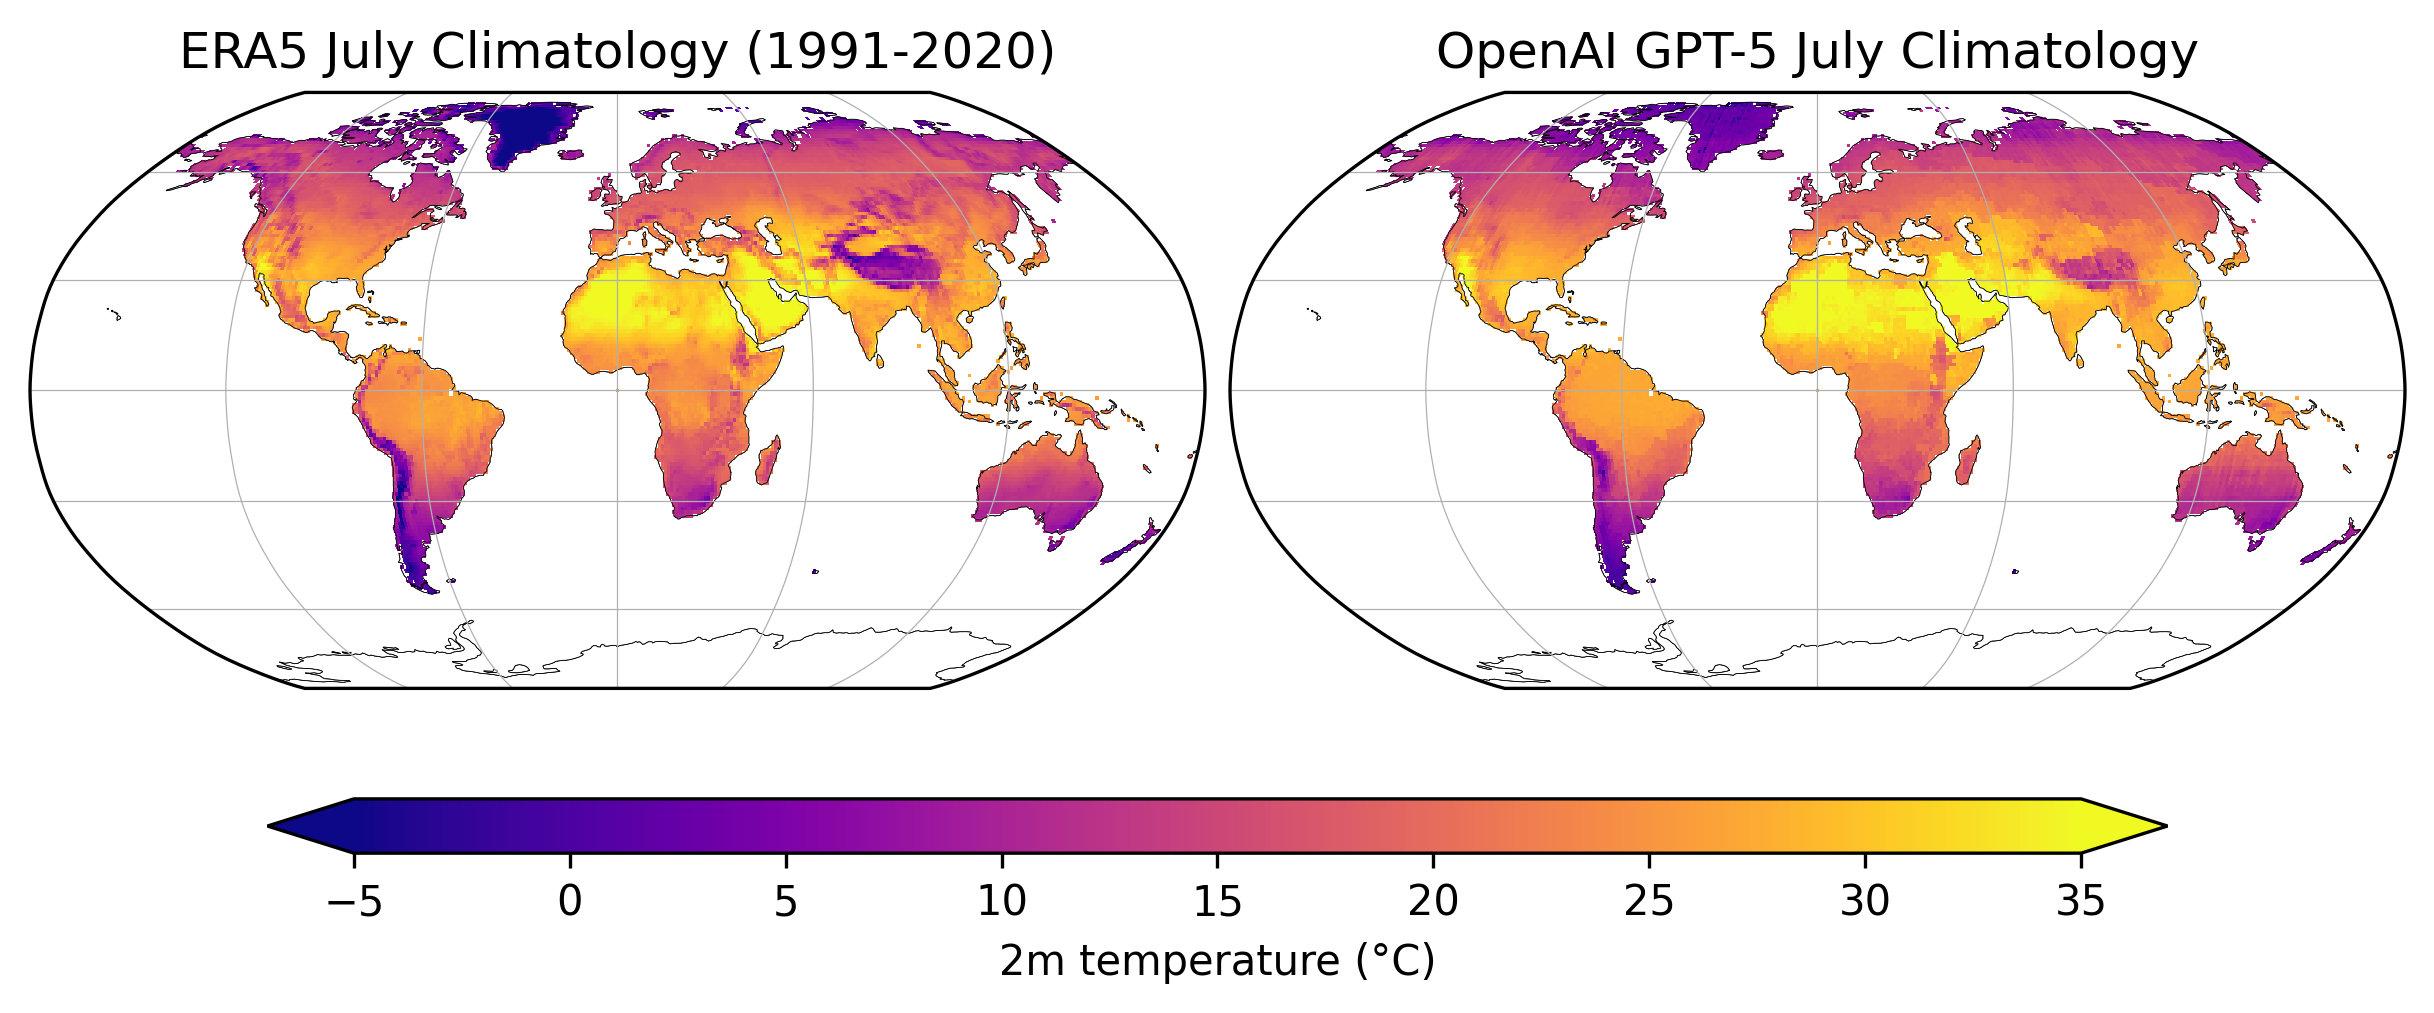
\includegraphics[width=1\linewidth]{Chapter4//figs/example_map.png}
    \caption{Mean July 2-m air temperature (1991-2020) from ERA5 reanalysis (left) and LLM GPT-5 predictions (right). Both panels are shown on a 1° grid.}
    \label{fig:july-climatology}
\end{figure}

The comparison was extended to all the model configurations included in the benchmark. Figure~\ref{fig:temperature-bias-maps} presents the reconstructed climatologies and their differences from ERA5, while Table~\ref{tab:llm-temperature-performance} and Figure~\ref{fig:bias_rmse_scatter} summarizes their global RMSE and mean bias. Across the configurations, RMSE ranges from \(3.5\,^{\circ}\mathrm{C}\) for GPT-5 to \(10.2\,^{\circ}\mathrm{C}\) for ClimateGPT 70B, with a median close to \(5\,^{\circ}\mathrm{C}\). Most models fall within the range of 3--\(6\,^{\circ}\mathrm{C}\). Changes in the sampling temperature have a much smaller effect. Moving from deterministic generation to a sampling temperature of 0.3 produces only marginal and inconsistent variations.

\begin{figure}[H]
    \centering
    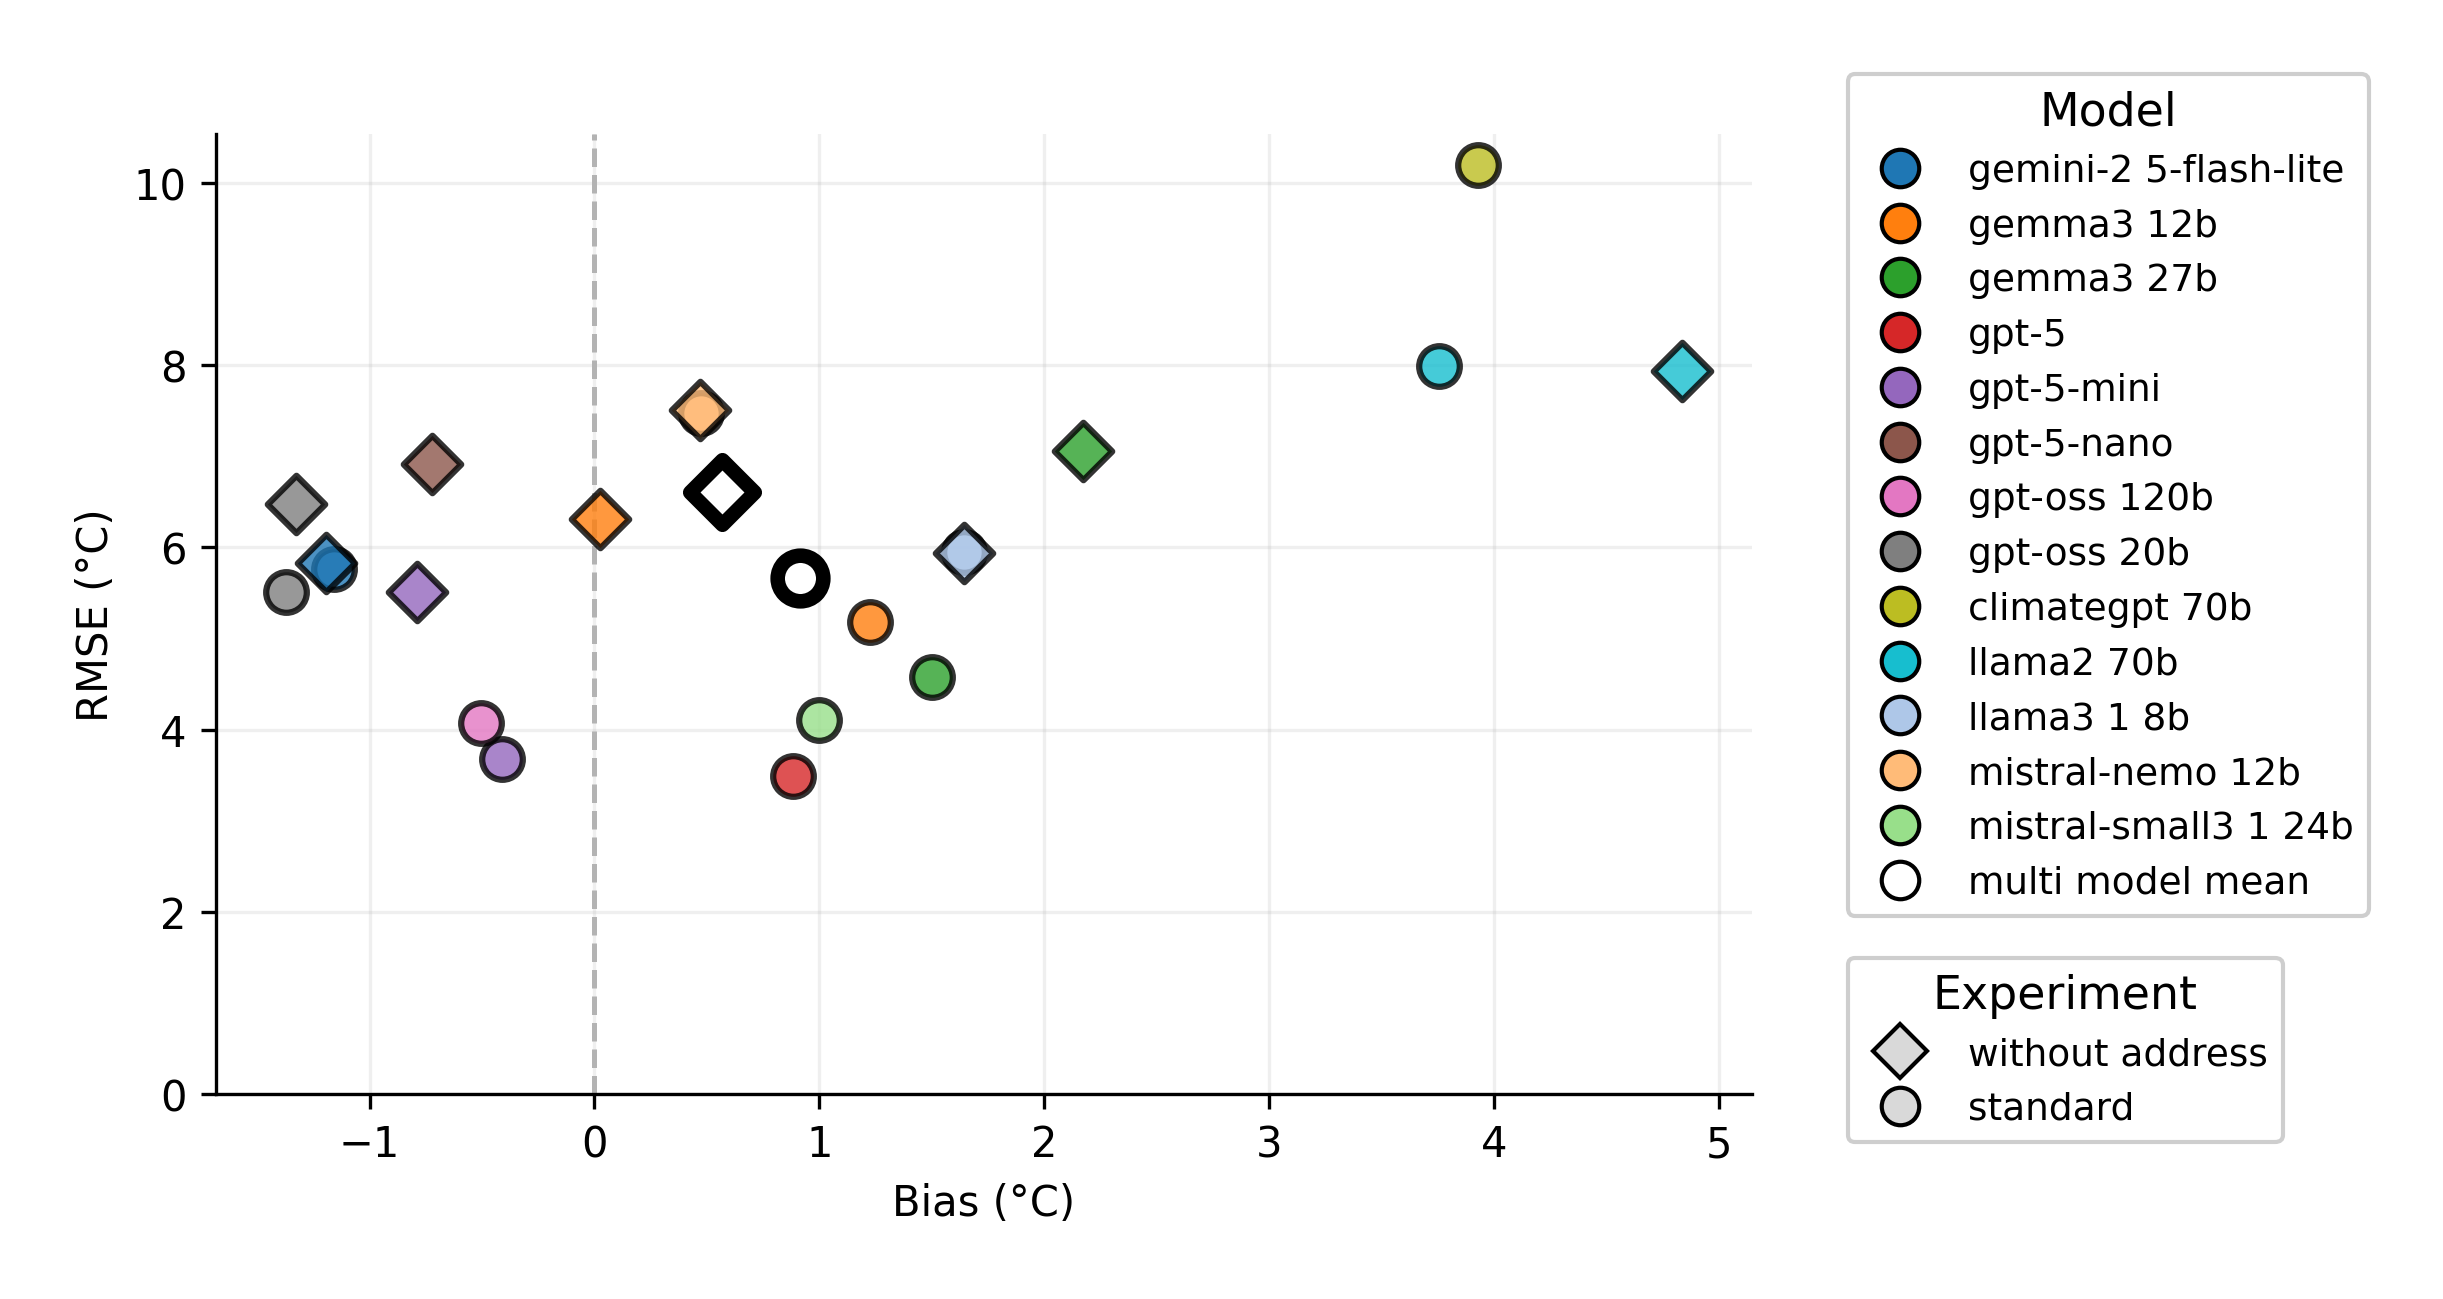
\includegraphics[width=1\linewidth]{Chapter4//figs/bias_rmse_scatter.png}
    \caption{Root-mean-square error (RMSE) against mean bias for LLM temperature
    predictions. All values are expressed in \(^{\circ}\mathrm{C}\). Only the simulation with \emph{temperature}=0 are shown, since setting \emph{temperature}=3 only produces small variations.}
    \label{fig:bias_rmse_scatter}
\end{figure}

The experiments show that the geographical information included in the prompt has a substantial influence on the results. Removing country, region, and city increases RMSE by an average of 27\%. For GPT-5 Mini, the error increases from 3.7 to \(5.6\,^{\circ}\mathrm{C}\); for Gemma 27B, it increases from 4.5 to \(7.1\,^{\circ}\mathrm{C}\); and for GPT-5 Nano, from 5.2 to \(6.9\,^{\circ}\mathrm{C}\). In contrast, some smaller models, including LLaMA 3.1 8B and Mistral Nemo 12B, show little sensitivity to the additional descriptors. This result suggests that coordinates alone are not an effective key to the climate information stored in many LLMs. Place names provide recognizable linguistic anchors that connect the query to geographical and climatic descriptions encountered during training. 

Mean biases are smaller than the corresponding RMSE values, since regional errors of opposite sign partly compensate when averaged over the global domain. Among the best configurations, they range from approximately \(-0.6\) to \(+0.9\,^{\circ}\mathrm{C}\), while the complete ensemble spans from \(-1.4\) to \(+4.8\,^{\circ}\mathrm{C}\). Interestingly, the sign of the bias also remains generally stable when the sampling configuration or the amount of geographical information in the prompt is changed, suggesting that warm or cold tendencies are characteristic of the models rather than consequences of individual prompt formulations.

% Prima pagina: pannelli (a)--(f)
\begin{figure}[p]
    \centering

    \mapmodel
        {Chapter4/figs/OpenAI GPT-5_map.png}
        {GPT-5}
    \hfill
    \mapmodel
        {Chapter4/figs/OpenAI GPT-5 Mini_map.png}
        {GPT-5 Mini}

    \medskip

    \mapmodel
        {Chapter4/figs/OpenAI GPT-5 Nano_map.png}
        {GPT-5 Nano}
    \hfill
    \mapmodel
        {Chapter4/figs/OpenAI GPT-OSS 20B_map.png}
        {GPT-OSS 20B}

    \medskip

    \mapmodel
        {Chapter4/figs/OpenAI GPT-OSS 120B_map.png}
        {GPT-OSS 120B}
    \hfill
    \mapmodel
        {Chapter4/figs/Gemini 2.5 Flash Lite_map.png}
        {Gemini 2.5 Flash Lite}

    \medskip
    
    \mapmodel
        {Chapter4/figs/Gemma3 12B_map.png}
        {Gemma 3 12B}
    \hfill
    \mapmodel
        {Chapter4/figs/Gemma3 27B_map.png}
        {Gemma 3 27B}

    

    \caption{
        Continues in the next page $\rightarrow$
    }
    \label{fig:temperature-bias-maps}
\end{figure}

% Seconda pagina: pannelli (g)--(m)
\begin{figure}[p]
    \ContinuedFloat
    \centering


    \mapmodel
        {Chapter4/figs/Mistral Nemo 12B_map.png}
        {Mistral Nemo 12B}
    \hfill
    \mapmodel
        {Chapter4/figs/Mistral Small3.1 24B_map.png}
        {Mistral Small 3.1 24B}

    \medskip

    \mapmodel
        {Chapter4/figs/LLaMA 2 70B_map.png}
        {LLaMA 2 70B}
    \hfill
    \mapmodel
        {Chapter4/figs/ClimateGPT 70B_map.png}
        {ClimateGPT 70B}

    \medskip

    \mapmodel
        {Chapter4/figs/LLaMA 3 1.8B_map.png}
        {LLaMA 3.1 8B}

    \caption[]{
        Spatial distribution of the July 2 m temperature bias relative to ERA5 for all the 13 models for the period 1991-2020. Only the configuration with \emph{temperature}=0 is reported, since setting \emph{temperature}=0 only produces small variations.
    }
\end{figure}

% Tabella risultati generali
\begin{longtable}{@{}lcc@{}}
    \caption{
        Root-mean-square error (RMSE) and mean bias for LLM temperature
        predictions. All values are expressed in \(^{\circ}\mathrm{C}\).
    }
    \label{tab:llm-temperature-performance}\\

    \toprule
    \textbf{Model/configuration}
    & \textbf{RMSE/bias (\(^{\circ}\mathrm{C}\))}
    & \textbf{RMSE/bias (\(^{\circ}\mathrm{C}\)) (No address)} \\
    \midrule
    \endfirsthead

    \multicolumn{3}{c}{%
        \tablename\ \thetable{} -- continued from previous page
    }\\
    \toprule
    \textbf{Model/configuration}
    & \textbf{RMSE/bias (\(^{\circ}\mathrm{C}\))}
    & \textbf{RMSE/bias (\(^{\circ}\mathrm{C}\)) (No address)} \\
    \midrule
    \endhead

    \midrule
    \multicolumn{3}{r}{Continued on next page}\\
    \endfoot

    \bottomrule
    \endlastfoot

    GPT-5, \(T=0.3\)
        & \(3.5 / 0.9\)
        & -- \\

    GPT-5 Mini, \(T=0.3\)
        & \(3.7 / {-0.4}\)
        & \(5.6 / {-0.8}\) \\

    GPT-5 Mini
        & \(3.7 / {-0.4}\)
        & -- \\

    GPT-OSS 120B, \(T=0.3\)
        & \(3.7 / {-0.6}\)
        & \(5.3 / {-0.6}\) \\

    GPT-OSS 120B
        & \(4.0 / {-0.4}\)
        & -- \\

    Mistral Small 3.1 24B, \(T=0.3\)
        & \(4.1 / 1.0\)
        & -- \\

    Mistral Small 3.1 24B
        & \(4.1 / 1.0\)
        & -- \\

    Gemma 27B, \(T=0.3\)
        & \(4.5 / 1.3\)
        & \(7.1 / 2.2\) \\

    Gemma 27B
        & \(4.6 / 1.5\)
        & -- \\

    GPT-OSS 20B, \(T=0.3\)
        & \(5.1 / {-1.3}\)
        & \(6.5 / {-1.3}\) \\

    Gemma 12B, \(T=0.3\)
        & \(5.2 / 1.1\)
        & -- \\

    Gemma 12B
        & \(5.2 / 1.2\)
        & \(6.3 / 0.0\) \\

    GPT-5 Nano, \(T=0.3\)
        & \(5.3 / {-0.8}\)
        & -- \\

    GPT-5 Nano
        & \(5.2 / {-0.8}\)
        & \(6.9 / {-0.7}\) \\

    GPT-OSS 20B
        & \(5.5 / {-1.4}\)
        & -- \\

    Gemini 2.5 Flash Lite, \(T=0.3\)
        & \(5.5 / {-1.2}\)
        & \(5.6 / {-1.2}\) \\

    Gemini 2.5 Flash Lite
        & \(5.8 / {-1.2}\)
        & \(5.8 / {-1.2}\) \\

    LLaMA 3.1 8B, \(T=0.3\)
        & \(5.9 / 1.8\)
        & \(5.9 / 1.8\) \\

    LLaMA 3.1 8B
        & \(6.0 / 1.6\)
        & \(5.9 / 1.6\) \\

    Mistral Nemo 12B, \(T=0.3\)
        & \(6.9 / 0.4\)
        & \(6.9 / 0.4\) \\

    Mistral Nemo 12B
        & \(7.5 / 0.5\)
        & \(7.5 / 0.5\) \\

    LLaMA 2 70B
        & \(8.0 / 3.8\)
        & \(7.9 / 4.8\) \\

    ClimateGPT 70B
        & \(10.2 / 3.9\)
        & -- \\

\end{longtable}

Model size provides a partial explanation for the differences in the performances. Within the same family, larger models generally perform better. GPT-5 and GPT-5 Mini outperform GPT-5 Nano, while GPT-OSS 120B improves on GPT-OSS 20B. However, this relationship does not hold across different model generations: LLaMA 3.1 8B outperforms the substantially larger LLaMA 2 70B by approximately \(2\,^{\circ}\mathrm{C}\). Model architecture, training data, and training procedure therefore appear to be at least as important as parameter count.

Domain specialization does not produce an advantage in this task. ClimateGPT 70B obtains the largest error in the ensemble, with an RMSE of \(10.2\,^{\circ}\mathrm{C}\), compared with \(8.0\,^{\circ}\mathrm{C}\) for the general-purpose LLaMA 2 70B from which it was derived. ClimateGPT was developed primarily for text-based climate question answering supported by retrieval, rather than for unaided numerical recall. Nevertheless, this comparison demonstrates that continued training on climate-related text does not necessarily improve the representation of quantitative climatological values and may alter numerical associations acquired by the original model.

The error maps show that he deviations are spatially coherent (Figure \ref{fig:temperature-bias-maps}). GPT-5 exhibits cold biases over parts of central Asia and South America and warm biases over Greenland and some areas of the Sahara. GPT-OSS 120B presents similarly coherent structures, although their sign differs in some regions. Mistral Small 3.1 24B and Gemma 27B show predominantly warm biases across large parts of the Northern Hemisphere mid-latitudes and colder biases in parts of the Southern Hemisphere.

A common feature across the models is the presence of particularly large errors over complex terrain. The Himalayas, the Tibetan Plateau, Greenland, the Andes, and other major mountain regions are systematically warmer in the LLM reconstructions than in ERA5. In these areas, the models reproduce the broad presence of a cold region but fail to represent the full magnitude of elevation cooling. By contrast, errors tend to be smaller over low-lying and densely populated areas.

The dependence on elevation is quantified in Table~\ref{tab:errors-by-altitude}, for four representative models. At elevations below 500 m, which contain 60.5\% of the evaluated land points, RMSE ranges from 1.9 to \(3.1\,^{\circ}\mathrm{C}\) across the four selected models. The error increases progressively with altitude, reaching 3.1--\(4.2\,^{\circ}\mathrm{C}\) between 1000 and 1500 m. A more pronounced deterioration occurs above 1500 m, where RMSE rises to 4.3--\(6.2\,^{\circ}\mathrm{C}\), depending on the model.

Above 2500 m, errors exceed \(7\,^{\circ}\mathrm{C}\) for all four models and are accompanied by warm biases ranging from approximately \(5\) to \(13\,^{\circ}\mathrm{C}\). Although only a relatively small fraction of the grid is located at these elevations, these points contribute disproportionately to the global error. Conversely, approximately 90\% of the evaluated locations lie below 1500 m, where the models perform considerably better. It is worth noting that ERA5, which is used here as the reference dataset, also has known limitations in representing data-sparse and high-elevation regions \citep{delhasse_brief_2020,munoz-sabater_era5-land_2021}. Therefore, the observed discrepancies cannot be attributed entirely to errors in the LLM estimates, as part of them may also reflect uncertainties in the reference data.

% Tabella risultati quota
\begin{table}[H]
    \centering
    \caption{
        RMSE and bias by altitude band for the selected models.
        The percentages indicate the fraction of grid cells belonging
        to each altitude band. All values are expressed in \(^{\circ}\mathrm{C}\).
    }
    \label{tab:errors-by-altitude}

    \resizebox{\textwidth}{!}{%
    \begin{tabular}{lrrrrrrrr}
        \toprule
        & \multicolumn{2}{c}{GPT-5}
        & \multicolumn{2}{c}{GPT-OSS 120B}
        & \multicolumn{2}{c}{Mistral Small 3.1 24B}
        & \multicolumn{2}{c}{Gemma 3 27B} \\
        \cmidrule(lr){2-3}
        \cmidrule(lr){4-5}
        \cmidrule(lr){6-7}
        \cmidrule(lr){8-9}

        \textbf{Altitude band}
        & \textbf{RMSE} & \textbf{Bias}
        & \textbf{RMSE} & \textbf{Bias}
        & \textbf{RMSE} & \textbf{Bias}
        & \textbf{RMSE} & \textbf{Bias} \\
        \midrule

        0--500 m (60.5\%)
        & 1.9 & -0.1
        & 3.1 & -1.4
        & 3.0 &  0.0
        & 3.1 &  0.2 \\

        500--1000 m (19.2\%)
        & 2.3 &  0.6
        & 3.3 & -0.3
        & 3.4 &  0.8
        & 3.3 &  1.1 \\

        1000--1500 m (10.3\%)
        & 3.1 & 1.5
        & 3.4 & 0.2
        & 3.9 & 1.9
        & 4.2 & 2.0 \\

        1500--2000 m (3.9\%)
        & 5.2 & 3.8
        & 4.3 & 0.9
        & 4.8 & 3.1
        & 6.2 & 4.1 \\

        2000--2500 m (2.3\%)
        & 8.5  & 7.3
        & 5.6  & 3.0
        & 7.0  & 5.8
        & 10.3 & 8.8 \\

        2500--3000 m (1.4\%)
        & 11.7 & 10.6
        & 7.4  & 5.1
        & 8.6  & 7.7
        & 14.1 & 12.8 \\

        3000--3500 m (0.6\%)
        & 12.4 & 10.9
        & 9.5  & 7.0
        & 11.7 & 10.4
        & 14.0 & 12.3 \\

        3500--4000 m (0.5\%)
        & 11.2 & 8.6
        & 10.3 & 5.4
        & 12.7 & 11.0
        & 11.5 & 9.7 \\

        \(>4000\) m (1.5\%)
        & 11.3 & 9.5
        & 9.5  & 5.7
        & 13.9 & 12.8
        & 11.6 & 9.2 \\

        \bottomrule
    \end{tabular}%
    }
\end{table}



As a last observation, the magnitude of some LLM errors is comparable to biases found when physical climate models are evaluated against reanalysis at similar spatial scales \citep{eyring_overview_2016}. This comparison provides a useful numerical reference but does not imply equivalence between the two types of model. Climate model errors arise from approximations in the representation of physical processes and boundary conditions, whereas LLM errors reflect incomplete or uneven statistical associations in their training material. Similar error magnitudes therefore have fundamentally different interpretations.




Overall, the experiment reveals a clear distinction between geographical plausibility and local quantitative reliability. Current LLMs encode enough climate information to reconstruct the broad spatial organization of July temperature and, in favorable conditions, to provide reasonable estimates for low-elevation and well-documented locations. Their errors nevertheless increase markedly where local temperature depends on geographical details that are not reliably represented in textual training data. The strong contribution of place names and the systematic difficulty over high terrain indicate that this capability should be interpreted as parametric recall supported by geographical associations, rather than as evidence of an internal physical model of the climate system.

\subsection{Climate Knowledge Across the Seasonal Cycle}

The previous analysis showed that LLMs encode a recognizable representation of the geographical distribution of July temperature. However, a single month cannot establish whether this knowledge extends to the complete annual cycle. To test this, the evaluation was repeated for all twelve calendar months using GPT-5, GPT-OSS 120B, Mistral Small 3.1 24B, and Gemma 27B. The experiment was conducted on the subset of 1,540 land points described in the previous section, with each model asked to return the twelve monthly climatological temperatures in a single response.

The extension to the annual cycle broadly confirms the conclusions obtained from the July experiment. As shown in Figure~\ref{fig:monthly-rmse}, the relative ranking of the four models is preserved across the year. When evaluated over all 18,480 point-month combinations, GPT-5 achieves the lowest RMSE, \(3.73\,^{\circ}\mathrm{C}\), followed by GPT-OSS 120B with \(4.00\,^{\circ}\mathrm{C}\), Mistral Small 3.1 24B with \(4.94\,^{\circ}\mathrm{C}\), and Gemma 27B with \(6.10\,^{\circ}\mathrm{C}\). The ability to reproduce the July climatology is therefore not an isolated result, but reflects a more general representation of the seasonal temperature cycle.

GPT-5 also exhibits the most stable performance throughout the year. Its monthly RMSE ranges from \(3.46\) to \(4.09\,^{\circ}\mathrm{C}\), with a mean annual bias of \(-0.33\,^{\circ}\mathrm{C}\). The other three models are warm-biased when evaluated across the full annual cycle, with biases ranging from \(+0.86\) to \(+1.77\,^{\circ}\mathrm{C}\). Their errors also display a more pronounced seasonal dependence, generally increasing during boreal autumn. Mistral Small 3.1 24B reaches an RMSE of \(6.22\,^{\circ}\mathrm{C}\) in November, while Gemma 27B reaches \(7.14\,^{\circ}\mathrm{C}\) in October.

These results indicate that the models encode the broad timing and direction of the seasonal cycle, including the reversal of seasons between the Northern and Southern Hemispheres. Nevertheless, the quantitative errors remain substantial. The ERA5 interannual variability calculated at the same locations averages \(2.00\,^{\circ}\mathrm{C}\) over the year, with larger values during boreal winter and smaller values during boreal summer. The monthly errors produced by the LLMs are therefore typically two to three times larger than the natural year-to-year variability of monthly temperature. A model may consequently reproduce the general form of the seasonal cycle while still providing climatological values that are unreliable for quantitative local applications.

\begin{figure}[H]
    \centering
    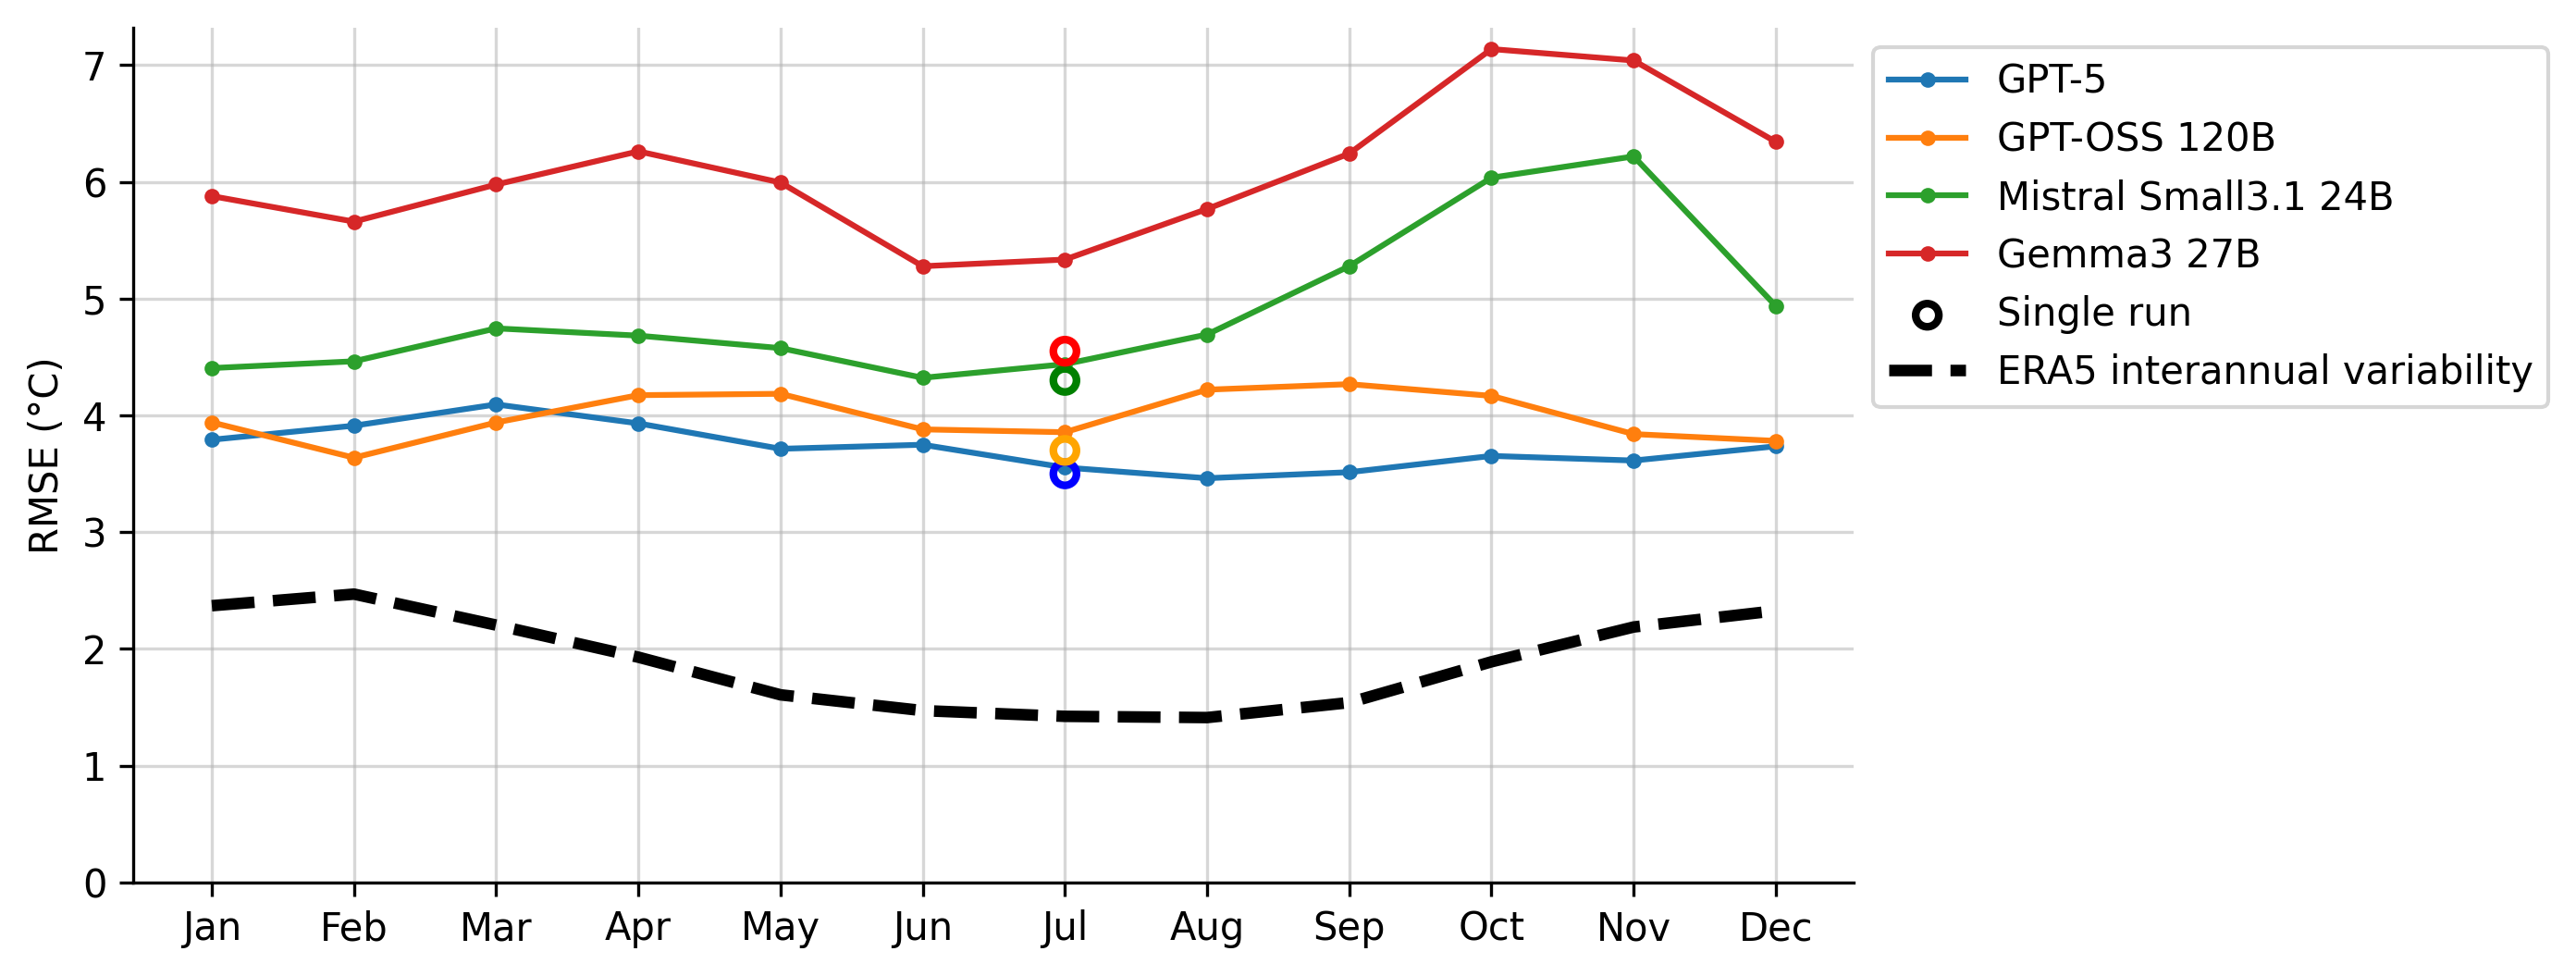
\includegraphics[width=\linewidth]{Chapter4/figs/seasonal_rmse.png}
    \caption{
        Monthly RMSE of closed-book LLM predictions of mean 2-m air temperature for 1991--2020 against ERA5. Results are shown for GPT-5, GPT-OSS 120B, Mistral Small 3.1 24B, and Gemma 27B at 1,540 land points. The dashed black line represents ERA5 interannual variability, while open circles show the corresponding results obtained from independent single month queries. All LLM experiments shown here use the default sampling configuration of the respective API.
    }
    \label{fig:monthly-rmse}
\end{figure}

Part of the difference between the July and annual experiments may be related to the structure of the query itself. In the main benchmark, the models were asked to provide only the July temperature. In the seasonal experiment, they had to return twelve coherent values in the same response. To separate the effect of this additional task complexity from differences in stored climatological information, the July value extracted from the joint twelve-month query was compared with the result of an independent single-month July query.

For GPT-5, the two formulations produce nearly identical results: the July RMSE is \(3.55\,^{\circ}\mathrm{C}\) in the joint query and \(3.59\,^{\circ}\mathrm{C}\) in the single-month query. The joint query increases RMSE by approximately \(0.2\,^{\circ}\mathrm{C}\) for GPT-OSS 120B and Mistral Small 3.1 24B. The largest difference is observed for Gemma 27B, whose July RMSE increases from \(4.55\) to \(5.34\,^{\circ}\mathrm{C}\). The weaker model is therefore more sensitive to the requirement of producing a complete and internally coherent annual cycle.

This comparison suggests that the seasonal errors combine two distinct limitations. The first concerns the climate information represented in the model parameters. The second concerns the ability of the model to retrieve and organize several related numerical values within a single response. This distinction is relevant for Climate Services, where LLMs may be required to communicate complete time series or sets of indicators rather than isolated values.

The robustness of these conclusions was further evaluated with respect to the sampling configuration and the reduced spatial domain. Figure~\ref{fig:sampling-sensitivity} compares the July results obtained using sampling temperatures of 0 and 0.3 with those obtained using the default setting of each API. Across the four models, changing the sampling configuration modifies RMSE by no more than \(0.45\,^{\circ}\mathrm{C}\) and mean bias by no more than \(0.18\,^{\circ}\mathrm{C}\). These changes are small compared with the differences between models.

GPT-OSS 120B shows the largest sensitivity, with RMSE decreasing from \(4.11\,^{\circ}\mathrm{C}\) under deterministic sampling to \(3.66\,^{\circ}\mathrm{C}\) using the API-default configuration. For the other three models, RMSE varies by \(0.15\,^{\circ}\mathrm{C}\) or less. The choice of sampling temperature therefore has only a secondary influence on the estimated climate knowledge and does not alter the relative performance of the models.

\begin{figure}[H]
    \centering
    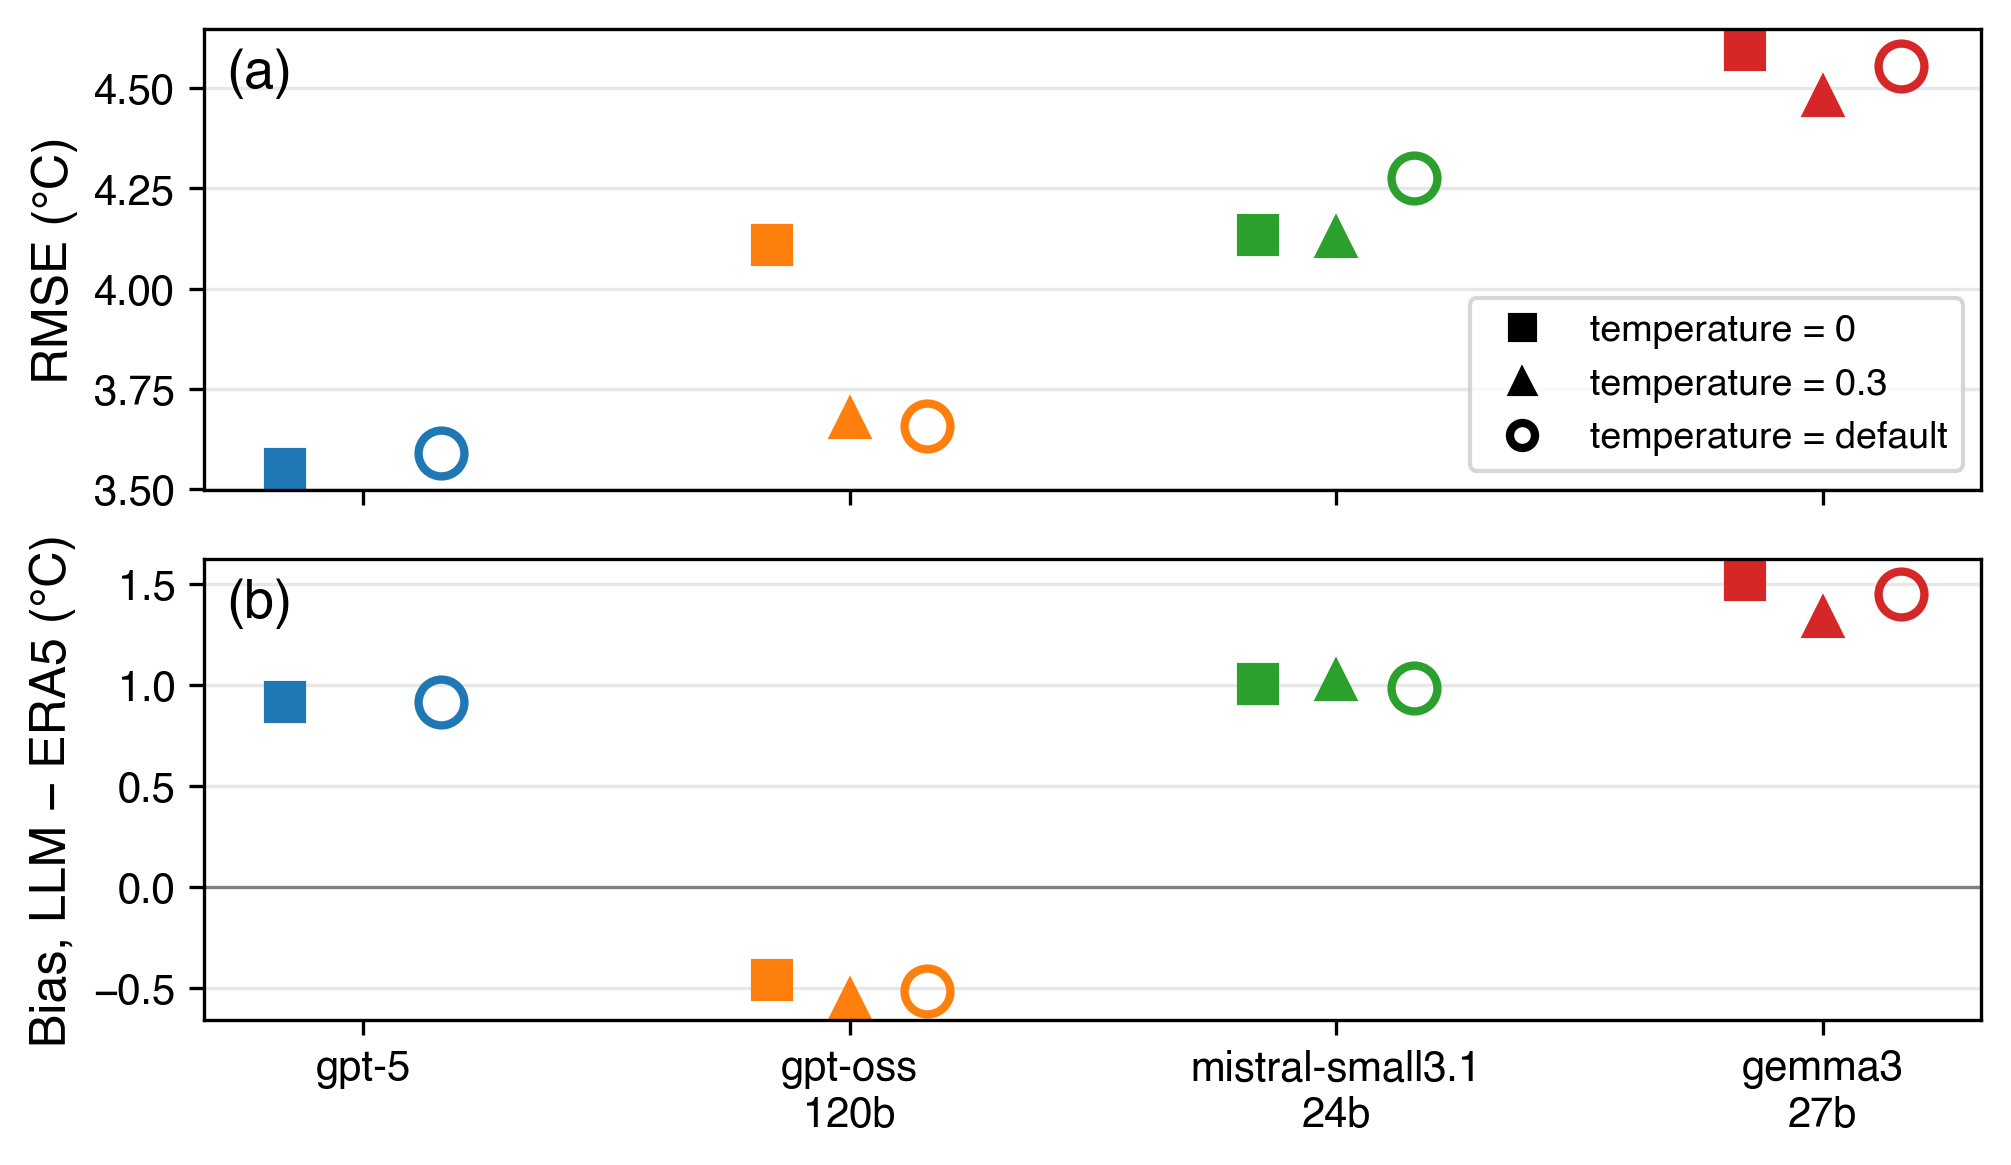
\includegraphics[width=0.75\linewidth]{Chapter4/figs/sampling_sensitivity.png}
    \caption{
        Sensitivity of July temperature performance to the sampling configuration on the 1,540-point subset. Panels show (a) RMSE and (b) mean bias relative to ERA5. Filled squares indicate sampling temperature 0, filled triangles indicate sampling temperature 0.3, and open circles indicate the default API configuration.
    }
    \label{fig:sampling-sensitivity}
\end{figure}

The subset used for the seasonal experiment also reproduces the results obtained over the complete global grid. At a sampling temperature of 0.3, GPT-OSS 120B has an RMSE of \(3.68\,^{\circ}\mathrm{C}\) on the subset and \(3.67\,^{\circ}\mathrm{C}\) on the complete grid. For Gemma 27B, the corresponding values are \(4.48\) and \(4.49\,^{\circ}\mathrm{C}\). The ten-percent subset can therefore be considered representative of the larger spatial experiment for the purpose of comparing monthly performance.

Overall, the seasonal extension reinforces the distinction between structural and quantitative climate knowledge. The evaluated LLMs reproduce the broad annual temperature cycle and maintain a relatively stable ranking across months. Their numerical errors, however, remain larger than the observed interannual variability, and weaker models become less reliable when several climatological values must be generated simultaneously. The results are robust to both the spatial subsampling and the sampling-temperature configuration, indicating that these limitations reflect the underlying models rather than specific experimental choices.




\subsection{Parametric Knowledge of Climate Change}

The previous experiments evaluated whether LLMs encode the present-day temperature climatology and its seasonal cycle. These quantities describe relatively stable characteristics of the climate system that are frequently associated with specific locations in textual sources. Representing climate change poses a different and more demanding problem. It requires the model not only to associate a location with a typical temperature, but also to distinguish between different historical periods and quantify how that temperature has changed over time.

To evaluate this capability, the models were asked to estimate the difference in mean July 2-m air temperature between 1950--1974 and 2000--2024. The resulting values were compared with the corresponding differences derived from ERA5. As in the previous experiments, the models operated in a closed-book setting and were not provided with external observations, reanalysis data, or time series from which the temperature change could be calculated. We repeated the experiment for GPT5, which acheved the best performances in the previous test, and Mistral Small 3.1 24b as representative of a small open source model.

At the global scale, the models reproduced the approximate magnitude of observed warming. The mean temperature change over ERA5 land points is \(1.05\,^{\circ}\mathrm{C}\), while GPT-5 estimates a global mean of approximately \(0.96\,^{\circ}\mathrm{C}\). Mistral Small 3.1 24B produces an average warming of approximately \(0.8\,^{\circ}\mathrm{C}\). These values indicate that information about the overall magnitude of recent global warming is represented in the parameters of the models.

This apparent agreement at the global level, however, does not extend to the geographical distribution of the change. Figure~\ref{fig:climate-change-map} compares the ERA5-derived temperature change with that estimated by GPT-5. The model produces some spatial variation, but the resulting pattern does not reproduce the regional structure found in ERA5. The agreement in the global mean therefore results from averaging geographically inconsistent estimates.

\begin{figure}[H]
    \centering
    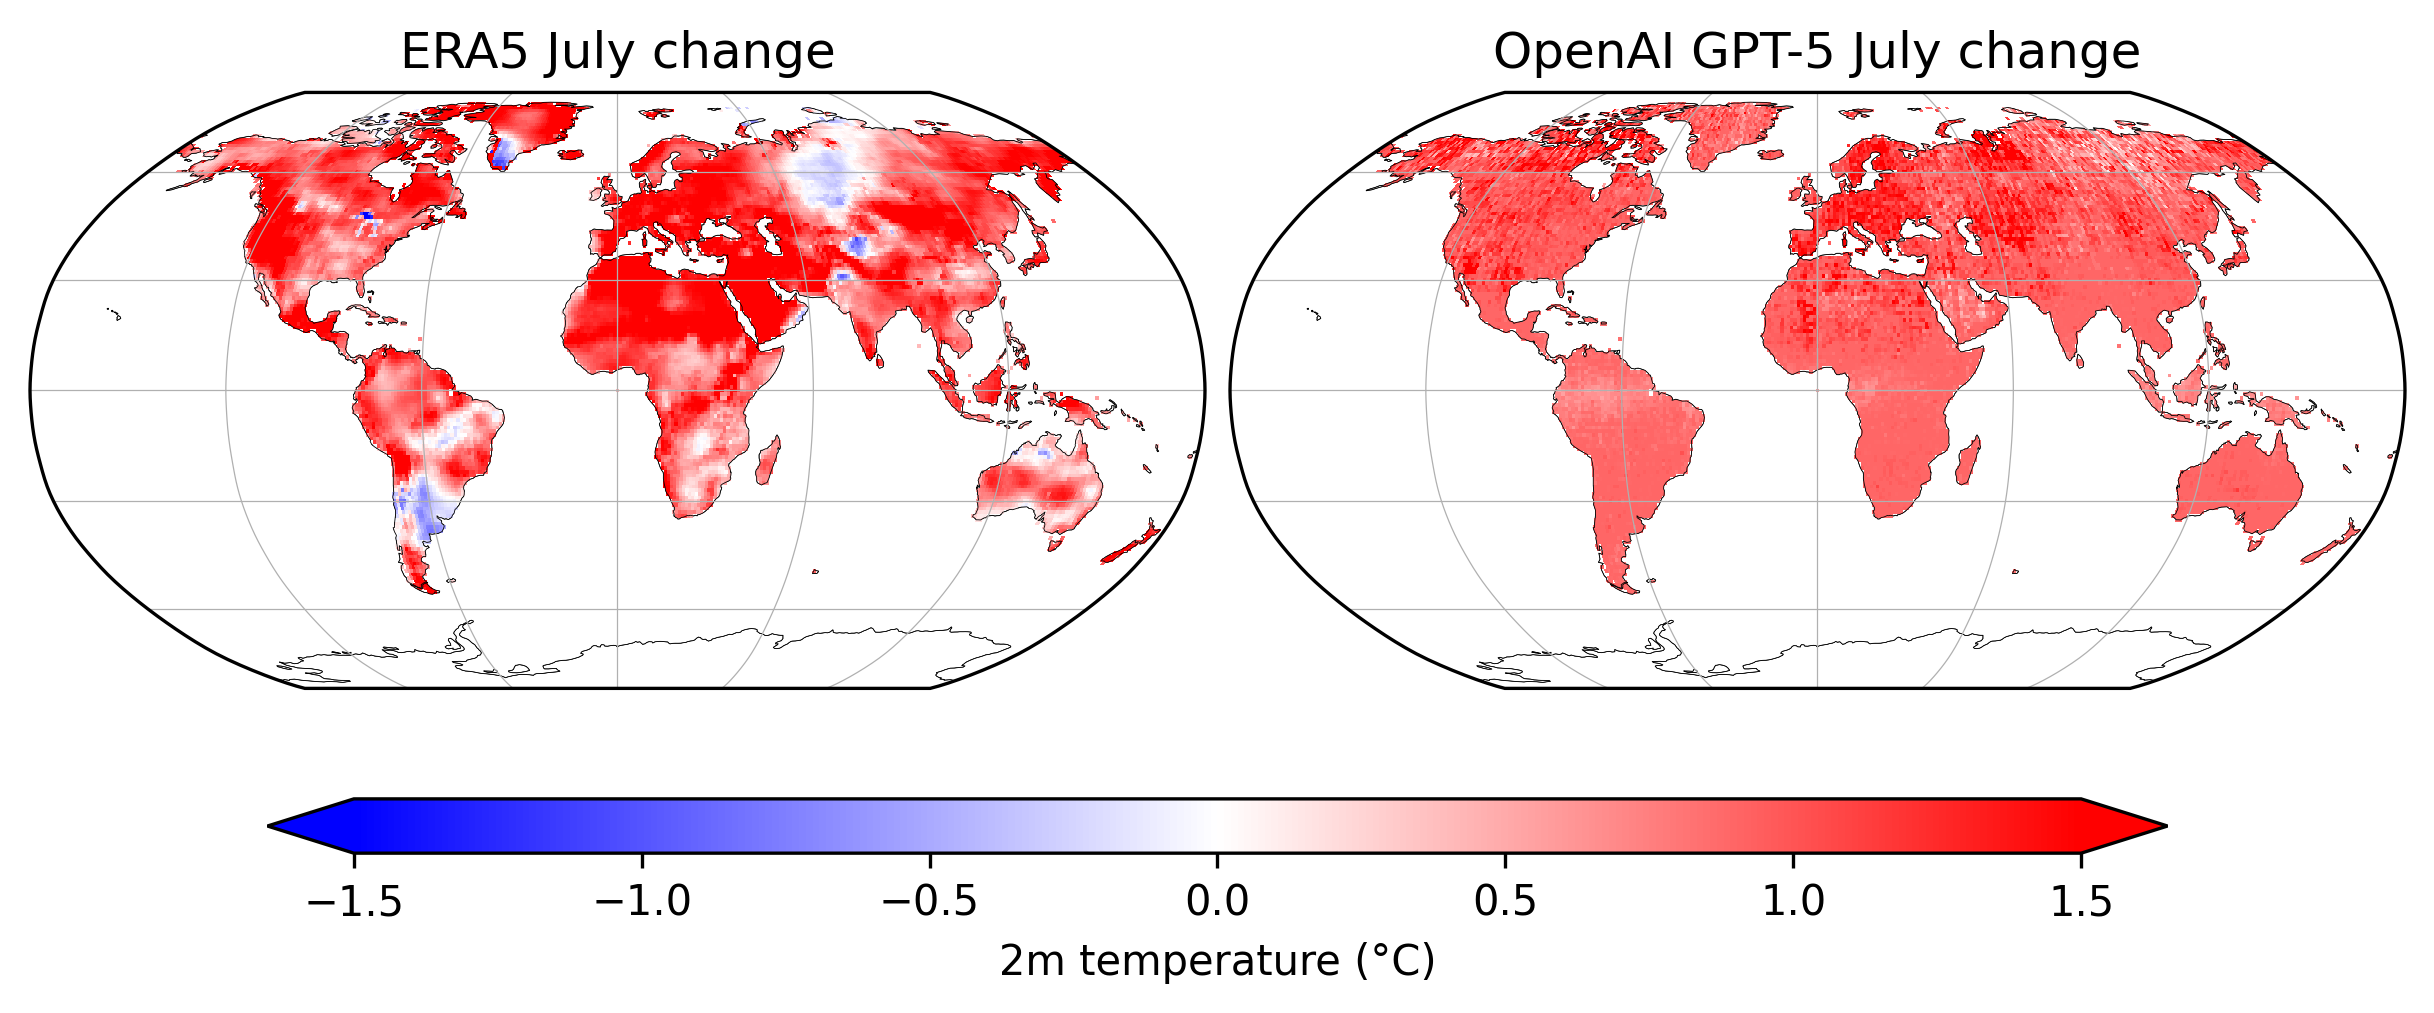
\includegraphics[width=0.75\linewidth]{Chapter4/figs/change_map.png}
    \caption{
        Change in mean July 2-m air temperature between 1950--1974
        and 2000--2024. The figure compares the change derived from
        ERA5 with the corresponding closed-book estimates produced
        by GPT-5.
    }
    \label{fig:climate-change-map}
\end{figure}

The spatial distribution of the errors for the two models is shown in Figure~\ref{fig:climate-change-bias}. Despite their different architectures, the models produce remarkably similar error patterns relative to ERA5. The absolute spatial correlation between each error field and the ERA5 change exceeds 0.90, whereas the change fields generated by the models correlate with ERA5 by less than 0.10. This occurs because both models produce nearly uniform warming maps centred around the approximate global mean value, with little meaningful regional variability. When these nearly constant estimates are compared with ERA5, the resulting error fields largely reproduce the spatial structure of the reference field, with the sign depending on the adopted bias convention. The similarity of the errors across models therefore does not indicate consistent geographical skill; rather, it reflects their common failure to represent the regional distribution of warming.

\begin{figure}[H]
    \centering
    \mapmodel
        {Chapter4/figs/change_bias_OpenAI GPT-5.png}
        {GPT-5}
    \hfill
    \mapmodel
        {Chapter4/figs/change_bias_Mistral Small 3.1 24b}
        {Mistral Small 3.1 24b}
    \caption{
        Spatial distribution of the bias in the estimated change in mean July 2-m air temperature between 1950--1974 and 2000--2024 for (a) GPT-5 and (b) Mistral Small 3.1 24B. Bias is defined as the LLM estimate minus the ERA5 change. The similar error patterns arise because both models produce nearly uniform warming fields, leaving the regional variability represented by ERA5 as the dominant structure in the residuals.
        }    
    \label{fig:climate-change-bias}
\end{figure}

The limitation is particularly evident for Mistral Small 3.1 24B, which returns an almost spatially uniform warming of approximately \(0.87\,^{\circ}\mathrm{C}\). GPT-5 estimates a similar global mean of \(0.96\,^{\circ}\mathrm{C}\), but produces a wider range of values across locations. In both cases, these averages are relatively close to the ERA5 land mean of \(1.05\,^{\circ}\mathrm{C}\), despite the poor correspondence of the individual grid-point estimates.

Figure~\ref{fig:q_q} separates the ability to reproduce the distribution of temperature changes from the ability to assign those changes to the correct locations. For GPT-5, the paired values show substantial variability around the global mean, and the quantile--quantile comparison indicates that the model reproduces part of the range found in ERA5. However, this distribution is compressed, particularly for the largest changes, and the weak point-wise relationship shows that the generated values are not associated with the correct geographical locations.

The limitation is more pronounced for Mistral Small 3.1 24B. Its paired values form an almost horizontal band around the model mean, while its quantiles vary only slightly across the much broader ERA5 distribution. The model therefore appears to apply approximately the same global warming value to almost every location. These results show that agreement in the global mean is not sufficient evidence of regional climate knowledge. GPT-5 generates some spatial variability without reproducing its geographical organization, whereas Mistral largely collapses the complete field towards a single global value.

\begin{figure}[H]
    \centering

    \begin{subfigure}{0.9\textwidth}
        \centering
        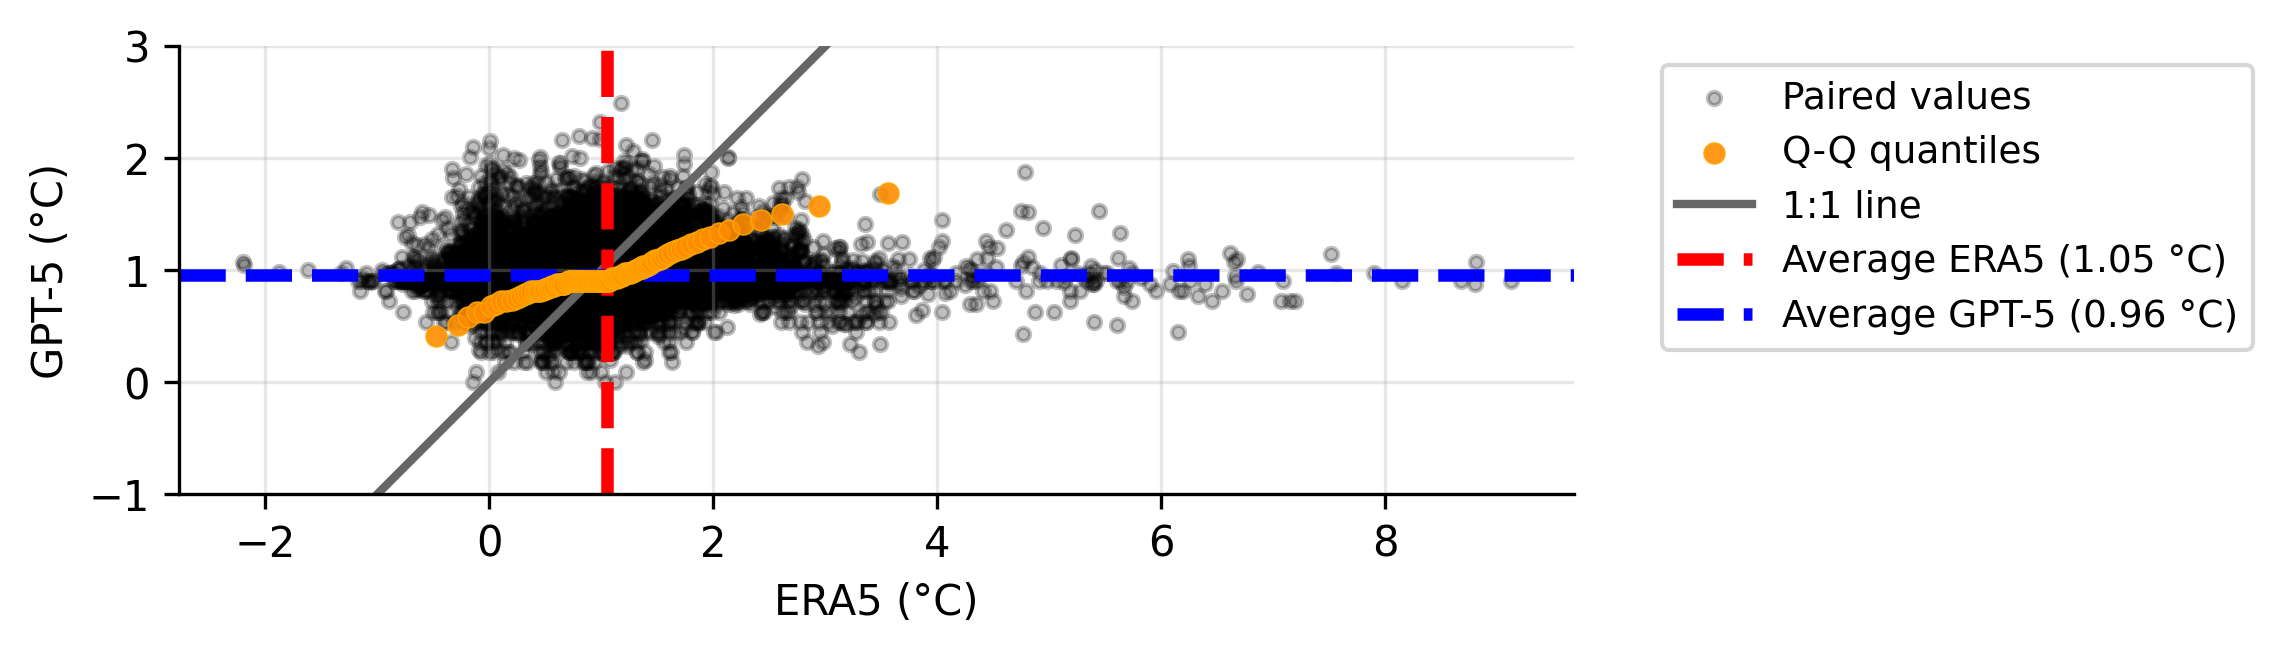
\includegraphics[width=\textwidth]{Chapter4/figs/change_q_q_OpenAI GPT-5.png}
        \caption{GPT-5}
        \label{fig:plot1}
    \end{subfigure}

    \vspace{0.5cm}

    \begin{subfigure}{0.9\textwidth}
        \centering
        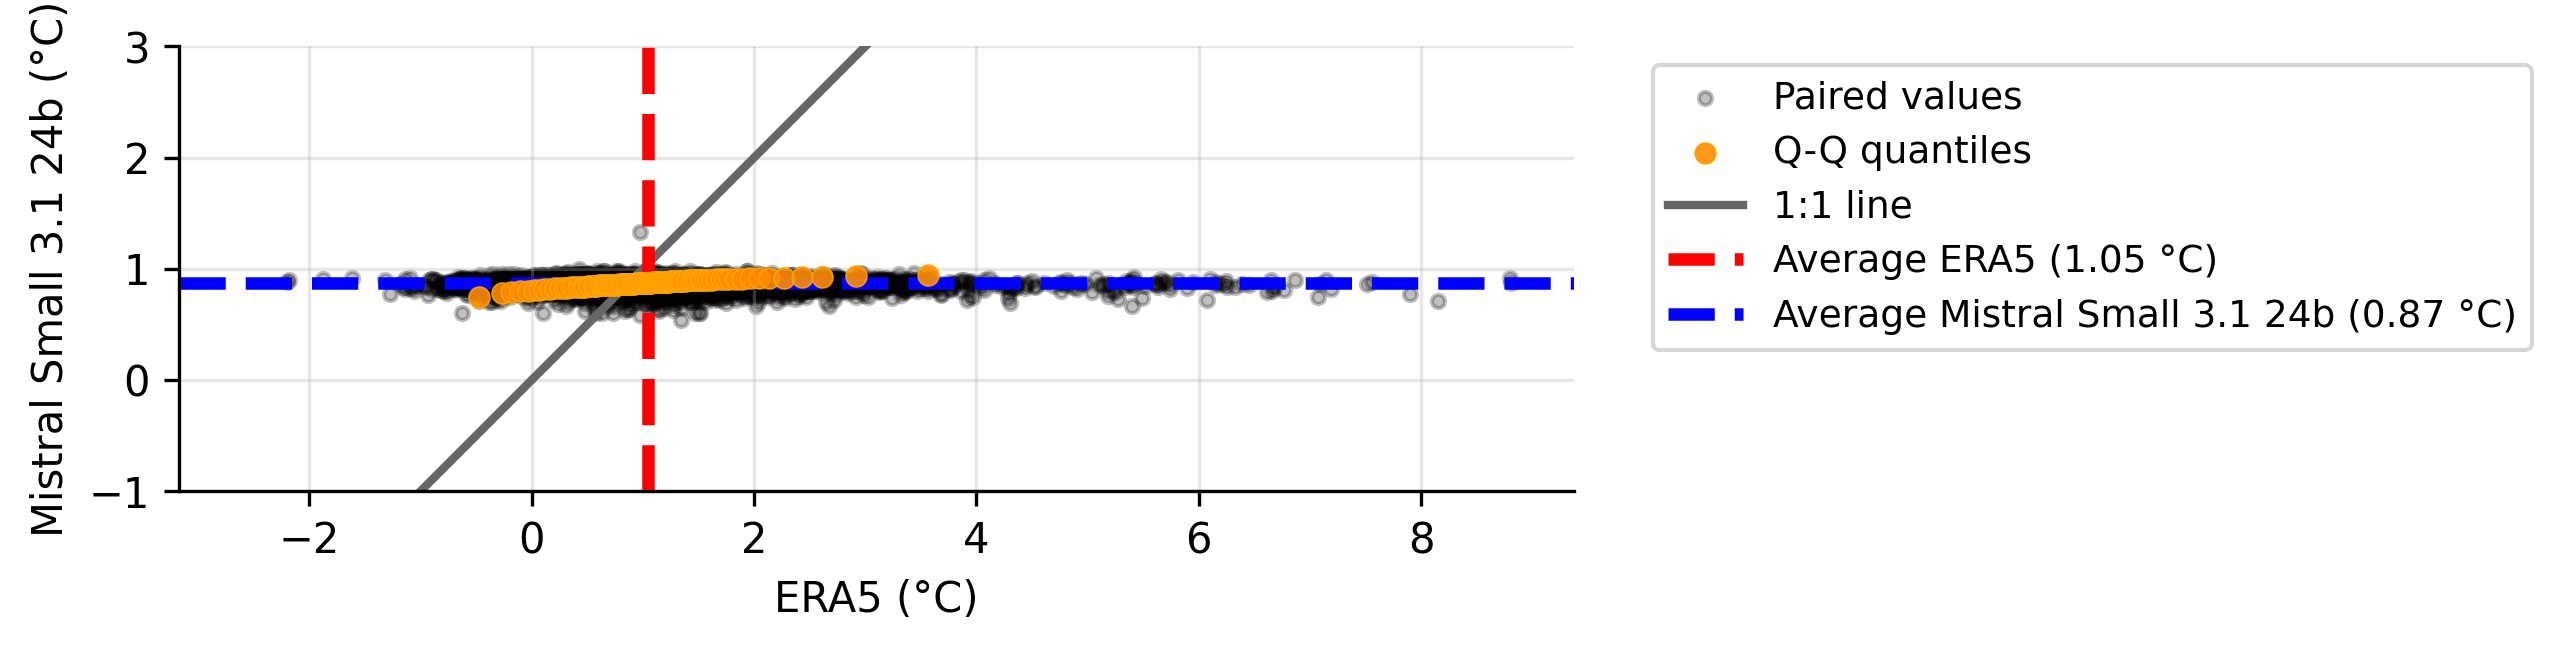
\includegraphics[width=\textwidth]{Chapter4/figs/change_q_q_Mistral Small 3.1 24b.png}
        \caption{Mistral Small 3.1 24b}
        \label{fig:plot2}
    \end{subfigure}

    \caption{
        Comparison between ERA5-derived and LLM-estimated changes in mean July 2-m air temperature between 1950--1974 and 2000--2024 for (a) GPT-5 and (b) Mistral Small 3.1 24B. Grey points show paired values at individual grid cells, while orange points compare the quantiles of the two distributions. The grey line represents perfect agreement, and the red and blue dashed lines indicate the ERA5 and LLM global means, respectively. GPT-5 produces a broader but compressed range of temperature changes, whereas Mistral Small 3.1 24B returns values strongly concentrated around its global mean.
        }
    \label{fig:q_q}
\end{figure}

A possible explanation for this difference between climatological means and climate change lies in how the relevant information is represented in textual training data. The present-day climate of a city or region is often described explicitly through statements about typical monthly temperatures. These statements can create direct associations between place names and climatological values. Local temperature changes, by contrast, are less frequently reported as explicit numerical facts and are more often contained in scientific datasets, figures, or specialized publications.

Reconstructing a local change would therefore require the model either to have encountered the exact value during training or to combine information referring to the same location at different times. The results provide no evidence that the evaluated LLMs can systematically perform this second operation. They do not appear to reconstruct an implicit local time series from separate pieces of information and then derive a consistent temperature difference from it.


\section{Discussion}

The experiments presented in this chapter provide a quantitative characterization of the climate information encoded in the parameters of contemporary LLMs. Taken together, the results reveal a consistent distinction between the ability to reproduce broad and frequently documented climatic regularities and the ability to provide accurate, geographically specific information. The models capture the general spatial organization of temperature, the annual cycle, and the approximate magnitude of global warming. Their reliability, however, decreases when the requested information depends on local geographical features or on the regional expression of temporal change.

This distinction is central to assessing the possible role of LLMs in Climate Services. A response may be globally plausible and linguistically convincing while remaining unsuitable for a local quantitative application.


\subsection{Parametric Recall versus Climate Understanding}

The ability of LLMs to reproduce the broad distribution of temperature demonstrates that their parameters contain a non-trivial representation of the Earth's climate. The models distinguish warm tropical and subtropical regions from colder high latitudes, reproduce the reversal of the seasonal cycle between hemispheres, and associate many locations with reasonable climatological values. This information is sufficiently structured to generate fields that resemble a physical climatology at the global scale.

However, these results should not be interpreted as evidence that LLMs possess an internal physical representation of the climate system. Unlike numerical climate models, they do not calculate temperature from governing equations, surface properties, atmospheric circulation, or energy exchanges. Their answers result from statistical associations learned during training. The fact that a generated field appears physically plausible does not establish whether the model has recalled an explicit value, combined multiple textual associations, or produced an estimate based on geographically related concepts.

The strong effect of geographical descriptors supports this interpretation. Adding country, region, and city names reduces RMSE by 27\% on average, even though the coordinates and the target location remain unchanged. Place names therefore appear to provide more effective access to parametric climate knowledge than numerical coordinates. This is consistent with the structure of textual training corpora, in which climate information is usually associated with recognizable geographical entities rather than latitude--longitude pairs. Widely documented locations consequently benefit from stronger linguistic associations, while remote, sparsely populated, and high-elevation regions are represented less reliably.

The errors over complex terrain further illustrate the difference between statistical recall and physical inference. An empirical or physically based model supplied with elevation could account for at least part of the expected temperature decrease with altitude. The evaluated LLMs instead produce increasingly warm estimates above 1500 m, despite correctly identifying many mountain regions as colder than their surroundings. They capture the qualitative association between mountains and lower temperatures but do not apply it with sufficient quantitative consistency.

The climate change experiment provides an even clearer example. The models reproduce the approximate magnitude of global warming, a value that is widely stated in scientific and public communication. They do not, however, reconstruct its regional distribution. Mistral Small 3.1 24B returns nearly the same warming at every location, while GPT-5 generates a broader range of values that remains geographically misaligned with ERA5. Parametric knowledge therefore preserves a widely communicated global statistic without encoding the local temporal information required to reconstruct the corresponding spatial field.

The comparison between ClimateGPT and its general-purpose base model leads to a related observation. Climate-specific continued training does not necessarily improve quantitative climate recall. ClimateGPT was designed primarily for textual climate question answering with retrieval augmentation, and its poorer performance in this benchmark does not imply that domain adaptation is generally ineffective. It does show, however, that exposure to additional climate discourse cannot be assumed to improve the representation of numerical climatologies. Textual specialization and quantitative recall are distinct capabilities and should be evaluated separately.

Similarly, model size alone does not determine performance. Larger variants generally perform better within the same family, but a newer 8-billion-parameter model can outperform an older 70-billion-parameter model. Architecture, training data, training procedures, and model generation appear to be at least as important as parameter count. For practical applications, reliability must therefore be established for the specific model and configuration being deployed rather than inferred from size or domain specialization.

The benchmark has several limitations that define the scope of these conclusions. It evaluates one variable, near-surface air temperature, using ERA5 as the principal reference. Temperature has a relatively regular spatial structure and is widely represented in public information. Variables such as precipitation, wind, and extremes may prove more difficult because their distributions are less smooth and their local values are less frequently reported. Conversely, the benchmark evaluates numerical recall rather than the complete range of capabilities of an LLM. It does not test whether models can correctly interpret climate data when those data are explicitly provided.

\subsection{The Need for Authoritative External Sources}

The limitations identified in this chapter do not imply that LLMs cannot contribute to Climate Services. Rather, they clarify the role that these models can perform reliably. Their principal strength lies in providing a flexible natural-language interface that can interpret user questions, explain concepts, organize information, and adapt its presentation to different audiences. They should not, however, be treated as autonomous repositories of local quantitative climate information.

For questions requiring exact climatological values, time series, trends, or projections, authoritative data should be obtained from external sources. Retrieval from scientific literature can provide traceable textual evidence, while access to climate databases and dedicated computational tools can supply numerical values derived from observations, reanalysis, or model simulations. Existing climate-oriented assistants demonstrate how LLMs can be connected to these resources \citep{vaghefi_chatclimate_2023,koldunov_local_2024}. In such systems, the language model mediates between the user and the information source rather than replacing that source.

A reliable system should also make the origin of its answers visible. At a minimum, quantitative climate information should be accompanied by the dataset or publication from which it was obtained, the reference period, the spatial and temporal resolution, and any relevant uncertainty or limitation. If access to the required source fails, the system should communicate that limitation rather than silently substitute a parametric estimate. The results of this chapter quantify the magnitude of the error that such a substitution can introduce.

Within the DIKW framework, this division of responsibilities clarifies the contribution of LLMs to the transition from information to knowledge. Climate datasets and scientific literature provide the evidence; computational tools extract or derive the requested information; and the LLM supports its interpretation, contextualization, and communication. 

The following chapter builds on this conclusion by introducing the concept of Augmented Language Models (ALMs). ALMs are LLMs that can connect to external documents, climate datasets, and analytical tools and generate their outputs based on the evidence provided by these sources. Grounding the generation process in authoritative sources addresses the limitations of generic parametric recall, but also introduces new challenges for output evaluation. The next chapter addresses this problem by examining how different augmentation strategies affect the epistemic quality of LLM-based Climate Services.